\documentclass[varwidth, border =7pt]{standalone}
\usepackage{tikz}

\begin{document}
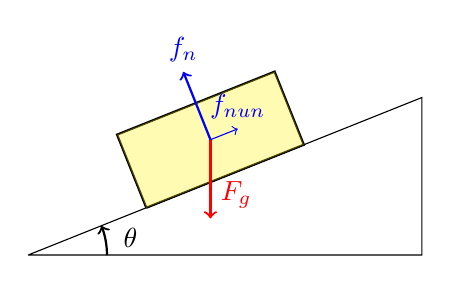
\begin{tikzpicture}

  %\draw [->] (0,0) -- (5.5,0 )node[anchor=west]{$x$}; %hnitakerfi
  %\draw [->] (0,0) -- (0, 3.3)node[anchor=south]{$y$}; %hnitakerfi
  \draw (0,0) -- (5,2) -- (5,0) -- (0,0); %skaplan
  \draw [thick](1.5, 0.6) -- (1.1286, 1.5285) -- (3.1286, 2.3285)-- (3.5,1.4) -- (1.5, 0.6); %kassi
  \fill [fill=yellow, opacity=0.3] (1.5, 0.6) -- (1.1286, 1.5285) -- (3.1286, 2.3285)-- (3.5,1.4) -- (1.5, 0.6); %kassi
  \draw [->, thick] (1,0) arc (0 : 21.8 : 1); %horn
  \draw (1.3,0.22) node { $\theta$}; %merking a horni
  %\draw [->, thick, red](1.5,1.1385) -- (0.5715, 0.7671);
  \draw [->, thick, red] (2.3143, 1.46424) -- (2.3143,0.46424) node[anchor=south west] {$F_g$}; % þyngdarkraftur
  \draw [->, thick, blue] (2.3143, 1.46424) -- (1.96947, 2.3263) node [anchor=south] {$f_n$}; % normalkraftur
  %\draw [red] (2.3143, 1.46424) -- (1.96947, 1.3263 ); %node [anchor] {\tiny $g_{x'}$};
  %\draw [red] (1.96947, 1.3263) -- (2.3143,0.46424); %
  %\draw [->, blue](3.2, 1.8185) -- (3.54483, 1.95644)  node[anchor=south] {$f_{nun}$} ;
  \draw [->, blue] (2.3143, 1.46424) -- (2.66146, 1.60216) node[anchor=south] {$f_{nun}$} ;

\end{tikzpicture}
\end{document}
